%% copyright 2020 Dony Darmawan Putra & Hasan Albinsaid

\documentclass[12pt, twoside , openright]{book}

%%%%%%%%%% instant packages %%%%%%%%%%
%% Copyright 2020 Dony Darmawan Putra & Hasan Albinsaid

%% for dots table of contents

\usepackage{booktabs}
\usepackage{titletoc}% http://ctan.org/pkg/titletoc
\usepackage{tocloft} %For TOC, TOF, TOT settings
\usepackage{zhnumber}
\usepackage[font=small]{caption}

\contentsmargin{0pt}
\renewcommand\contentspage{\thecontentspage}

\dottedcontents{section}[2.3em]{}{2.3em}{5pt}
\dottedcontents{subsection}[5.5em]{}{3.2em}{5pt}


\titlecontents*{chapter}% <section-type>
[0pt]% <left>
{}% <above-code>
{\bfseries\chaptername\ \thecontentslabel\quad}% <numbered-entry-format>
{}% <numberless-entry-format>
{\bfseries\dotfill\contentspage\\\vspace{0mm}}% <filler-page-format> 

\titlecontents*{section}% <section-type>
[0pt]% <left>
{}% <above-code>
{\bfseries\ \thecontentslabel\quad}% <numbered-entry-format>
{}% <numberless-entry-format>
{\bfseries\dotfill\contentspage\\\vspace{0mm}}% <filler-page-format> 

\titlecontents*{subsection}% <section-type>
[0pt]% <left>
{}% <above-code>
{\hspace{2mm}\bfseries\ \thecontentslabel\quad}% <numbered-entry-format>
{}% <numberless-entry-format>
{\bfseries\dotfill\contentspage\\\vspace{0mm}}% <filler-page-format> 

\newcommand*{\noaddvspace}{\renewcommand*{\addvspace}[1]{}}
\addtocontents{lof}{\protect\noaddvspace}
\addtocontents{lof}{\linespread{1}\selectfont}
\addtocontents{lot}{\protect\noaddvspace}
\addtocontents{lot}{\linespread{1}\selectfont}

%% Arabic Text
%% for Chinese typing
\usepackage{xeCJK}
\usepackage{ctex}
\setCJKmainfont{BiauKai}                    
\setCJKmonofont{BiauKai}

%% for sections
\usepackage{mfirstuc}

%% for images
\usepackage{graphicx}
\graphicspath{ {Images/} }
\usepackage{caption}
\usepackage{subcaption}
\renewcommand{\figurename}{圖}

%%table
\renewcommand{\tablename}{表}

%%  for paper size and margins
\usepackage[a4paper,top=2.54cm,bottom=2.54cm, left=3cm, right=3cm]{geometry}


%% for paragraph
%paragraph indentation
\usepackage{indentfirst}
\setlength{\parindent}{4em} 

%paragraph spacing
\setlength{\parskip}{1em}

%Line spacing
\renewcommand{\baselinestretch}{2}

%% for font size
\usepackage{setspace}
\usepackage{blindtext}
\newcommand{\bigsize}{\fontsize{16pt}{20pt}\selectfont}
\newcommand{\chinnesesize}{\fontsize{18pt}{20pt}\selectfont}

%% for header and footer
\usepackage{blindtext}
\pagestyle{plain}


%% for references
\usepackage[square,numbers]{natbib}
\renewcommand{\bibsection}{}

%% for chapter title
\renewcommand{\chaptername}{}
\renewcommand{\thechapter}{第\chinese{chapter}章}
\renewcommand{\thesection}{\arabic{chapter}.\arabic{section}}
\renewcommand{\thesubsection}{\arabic{chapter}.\arabic{section}.\arabic{subsection}}

\usepackage{titlesec}
\titleformat{\chapter}{\center\Large}{\thechapter}{1em}{}
\titlespacing*{\section}
{0pt}{0pt}{0pt}
\titlespacing*{\subsection}
{0pt}{0pt}{0pt}

%TOC
\renewcommand{\contentsname}{\hfill\bfseries\LARGE 目\hspace{1em}錄 \hfill}
\renewcommand{\cftaftertoctitle}{\hfill}
%TOF
\renewcommand{\listfigurename}{\hfill\bfseries\LARGE 圖\hspace{1em}次 \hfill}
\addtolength{\cftfignumwidth}{30pt}% More space
\DeclareCaptionListFormat{figprefix}{#1\figurename~#2}
\captionsetup[figure]{listformat=figprefix}
\renewcommand{\thefigure}{\arabic{chapter}-\arabic{figure}} %Add "-" dash in TOF
%TOT
\renewcommand{\listtablename}{\hfill\bfseries\LARGE 表\hspace{1em}次 \hfill}
\addtolength{\cfttabnumwidth}{30pt}% More space
\DeclareCaptionListFormat{tabprefix}{#1\tablename~#2}
\captionsetup[table]{listformat=tabprefix}
\renewcommand{\thetable}{\arabic{chapter}-\arabic{table}} %Add "-" dash in TOT


%%For background image
\usepackage[pages=some,scale=1,angle=0,opacity=1.0]{background}
\newcommand\BackImage[2][scale=1]{%
	\BgThispage
	\backgroundsetup{
		contents={\includegraphics[#1]{#2}}
	}
}


%% Algorithm    
\usepackage{algorithmic}
\usepackage{amsmath,amssymb,amsfonts}
\usepackage{mathtools}
\renewcommand{\theequation}{\arabic{chapter}.\arabic{equation}}
\usepackage{algorithm}
\renewcommand{\thealgorithm}{\arabic{chapter}.\arabic{algorithm}}
% \usepackage[linesnumbered,ruled,vlined,algochapter]{algorithm2e}
\usepackage{varioref}
\usepackage{hyperref}


%% Math Set Symbol
\usepackage{newtxmath}


%%%%%%%%%%%%%%%%%%%%%%%%%%%%%%%%%%%%%%%%
%%%%%%%%%% for body of document %%%%%%%%%%
%%%%%%%%%%%%%%%%%%%%%%%%%%%%%%%%%%%%%%%%
\begin{document}
	
	%%%%%%%%%% cover %%%%%%%%%%
	\thispagestyle{empty}
	\begin{center}
		\onehalfspacing
		
\includegraphics[width=0.205\textwidth]{logo_nsysu_thesis}
		
		{\chinnesesize 國立中山大學 Your Departement Chinese Name %%NSYSU Your Departement Name
			
			碩士論文} %%Master Thesis
		
		{\bigsize Your Departement Name\\National Sun Yat-sen University\\}
		{\bigsize Master Thesis\\}
		
		\vspace{2cm}
		{\chinnesesize Chinese Thesis Title\\}
		{\bigsize Thesis Title\\}
		\vspace{2cm}
		{\bigsize \hspace{0pt} 研究生：Your Chinese Name\\ %You can arrange the position manually by change hspace value
			\hspace{70pt} Your Name\\ %You can arrange the position manually by change hspace value
			\hspace{0pt} 指導教授：Advisor Chinese Name\\ %You can arrange the position manually by change hspace value
			\hspace{130pt}Advisor Name \\%You can arrange the position manually by change hspace value
		}
		
		\vspace{1.5cm}
		
		{\bigsize 中華民國109年1月\\
			January 2020\\
			
		}
	\end{center}
	

	\thispagestyle{empty}
	\clearpage
	\pagenumbering{roman}
	
	
	
	%%%%%%%%%% for thesis Validation Letter %%%%%%%%%%
	\addcontentsline{toc}{chapter}{論文審定書}
	\begin{center}
		{\chinnesesize 論文審定書 }
	\end{center}
	Validation letter
	\clearpage
	
	%%%%%%%%%% acknowledgment %%%%%%%%%%
	\phantomsection
	\addcontentsline{toc}{chapter}{銘謝}
	\begin{center}
		{\chinnesesize 銘謝}
	\end{center}
	
	"The most loved Man/Woman by Allah is the most beneficial to humans  beings.." (Narrated by Ath-Thabrani in Al Mu'jam Al Kabir no. 13280).
	
	Hopefully, this NSYSU Thesis LaTEX template can be useful for all of us, and you'll get the best results for your thesis.
	
	\noindent
	作者：
	
	\vspace{-2em}
	- 姓名
	\noindent \\
	日期：

	\vspace{-2em}
	- 
	
	
	\clearpage
	
	
	%%%%%%%%%% chinnese abstract %%%%%%%%%%
	\phantomsection
	\addcontentsline{toc}{chapter}{摘 要}
	\begin{center}
		{\chinnesesize 摘 要}
	\end{center}
	This is Abstract, but in chinese language. \blindtext[1]
	\clearpage
	
	
	
	
	
	%%%%%%%%%% english abstract %%%%%%%%%%
	\phantomsection
	\addcontentsline{toc}{chapter}{Abstract}
	\begin{center}
		{\chinnesesize Abstract}
	\end{center}
	
	This is Abstract. \blindtext[1]
	
	\BackImage[trim=0 +12cm 0 0, width=15.5em]{watermark.jpg} %watermark e-thesis (optional, usualy when we need to give to library)
	
	\noindent Keywords: keyword1, keyword2, keyword3.
	\clearpage
	
	
	
	
	%%%%%%%%%%
	\tableofcontents
	\clearpage
	
	
	
	
	%%%%%%%%%%
	\listoffigures
	\clearpage
	
	
	%%%%%%%%%%
	\listoftables
	\let \cleardoublepage \clearpage
	%%%%%%%%%%%%%%%%%%%%%%%%%%%%%%%%%%%%%
	%%%%%%%%%%for Main Contents%%%%%%%%%%
	%%%%%%%%%%%%%%%%%%%%%%%%%%%%%%%%%%%%%
	\mainmatter
	
	%%%%%%%%%%First Chapter%%%%%%%%%%
	\chapter{章節標題測試}
	This is your introduction. You can put the citation as this example \cite{CpLi}. For adding reference you can open bibliography file "references.bib" and paste the BibTeX into that file, to make it more clear you can see the example of BibTex in this link : \href{https://www.youtube.com/watch?v=SsJSR2b4_qc&t=107s}{Import BibTeX from Google Scholar}
	
	\blindtext[2] %<-this is dummy text
	
	
	
	
	
	%%%%%%%%%%Second Chapter%%%%%%%%%%
	\chapter{Second Chapter}
	This is your second chapter, the example for citation \cite{Ymc}. \blindtext[1]
	
	You can add figure, so it will show as Figure \ref{fig:figure_ref}
	\begin{figure}[h]
		\centerline{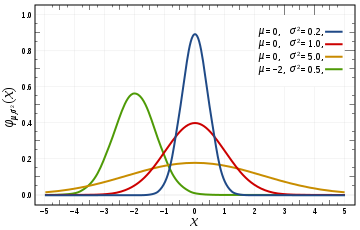
\includegraphics[width=0.5\columnwidth]{Images/gambar.png}}
		\caption{Gaussian distribution1}
		\label{fig:figure_ref}
	\end{figure}
	
	
	\section{小章節標題測試}\label{sub_chapter21}
	This is your sub chapter, the example for citation \cite{latexcompanion}. \blindtext[1].
	\begin{equation}
		\label{index_eq}
		(\hat{n})=\operatorname*{arg\,max}_{n\in \{1,\dots,M\}}(\mathbf{X}_{n})
	\end{equation}
	This is the example of equation, expressed as eq. \ref{index_eq}
	
	% \SetKwInput{KwInput}{Input}
	% \SetKwInput{KwOutput}{Output}  
	% \begin{algorithm}
	% 	%\DontPrintSemicolon
	% 	\KwInput{$\mathbf{A}$,$\mathbf{B}$}
	% 	\For{$j\gets1$ to $N_s$ by $1$}{
	% 		\For{$i\gets1$ to $N$ by $1$}{
	% 			$\mathbf{A}[i,j]=i+j$
	% 		}
	% 	}
	% 	$\mathbf{C}=\mathbf{A}+\mathbf{B}$
		
	% 	\KwOutput{Matrix result $\mathbf{C}$ }
	% 	\caption{The example of algorithm}
	% \end{algorithm}

	\begin{algorithm}
		\caption{test}
	\end{algorithm}
	
	
	\section{Sub-chapter}\label{sub_chapter22}
	This is your sub chapter. \blindtext[2]
	\begin{figure}[h]
		\centerline{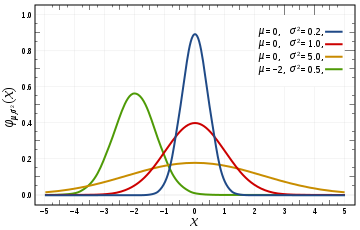
\includegraphics[width=0.5\columnwidth]{Images/gambar.png}}
		\caption{Gaussian distribution2}
		\label{fig:figure_ref2}
	\end{figure}
	
	
	
	
	%%%%%%%%%%Third Chapter%%%%%%%%%%
	\chapter{Third Chapter}
	This is your third chapter. \blindtext[1] 
	
	\section{Sub-chapter}\label{sub_chapter31}
	This is your sub chapter. \blindtext[1] You can add table, so it will show as Table \ref{table:table1}
	
	\begin{table}[h!]
		\begin{center}
			\caption{This is the example of table1}
			\label{table:table1}
			\begin{tabular}{|l|c|c|c|}
				\hline
				\textbf{Layer} & \textbf{Col1} & \textbf{Col2} \\ % <-- added & and content for each column
				\hline
				Row1 & content & content \\ % <--
				Row2 & a & b \\ % <--
				Row3 & c & d \\ % <--
				Row4 & e & f \\ % <--
				\hline
			\end{tabular}
		\end{center}
	\end{table}
	
	\section{Sub-chapter}\label{sub_chapter32}
	This is your sub chapter. \blindtext[2]
	\begin{table}[h!]
		\begin{center}
			\caption{This is the example of table2}
			\label{table:table2}
			\begin{tabular}{|l|c|c|c|}
				\hline
				\textbf{Layer} & \textbf{Col1} & \textbf{Col2} \\ % <-- added & and content for each column
				\hline
				Row1 & content & content \\ % <--
				Row2 & a & b \\ % <--
				Row3 & c & d \\ % <--
				\hline
			\end{tabular}
		\end{center}
	\end{table}
	
	
	
	
	\chapter{Conclusion}
	The conclusion is... \blindtext[1] %<-this is dummy text
	\clearpage
	
	%% for Reference
	\phantomsection
	\addcontentsline{toc}{chapter}{參考文獻}
	\begin{center}
		{\chinnesesize 參考文獻}
	\end{center}
	\bibliographystyle{IEEETran}
	\bibliography{references}
	
\end{document}